\chapter{序論}
\newpage
\section{研究背景}
日本の少子高齢化社会は今後益々深刻化するとされており, 高齢者の健康を考えることが今までにないほど重要になっている. 平成30年5月時点で日本の総人口は1億2644万6千人, 65歳以上の人口は3541万人であった. 前年度同日と比較すると総人口は25万8千人減少した一方で, 65歳以上の人口は46万8千人増加した\cite{jinkou}. 要介護認定者数は平成30年8月時点で659.2万人であり前年度の同月と比較して20万人増加している\cite{youkaigo1}\cite{youkaigo2}. \figref{kaigo}は要介護者を対象に要介護に至った主な原因を調査したものである. 認知症が18.7\%で最多, 次いで脳血管疾患(脳卒中)が15.1\%, 高齢による衰弱が13.8\%, 骨折や転倒が12.5\%であった\cite{kaigogenin}. 高齢者の要介護者が増加することは高齢者の生活水準を低下させ, 生き方の多様性を狭めることは勿論, 国の医療費負担の増加, 医療業界における人員不足など様々な社会問題を引き起こす. そこで本研究では高齢者に占める要介護者の減少させるために, 高齢者の寝たきりを予防するリング型アレイ超音波診断装置の開発を目標とする. 中でも認知症や脳血管疾患に比べて予防がしやすいという点から, 骨折や転倒を予防する手法を考案する. 
\\\ \ 骨折や転倒の原因としては, 脳の衰えと下肢組織の衰えが考えられるが, 本研究では下肢組織の衰えに着目する. 高齢者と若年者の下肢組織についてには比較検討されている. 池添冬芽らは, 加齢に伴ってヒト骨格筋においては筋張力が低下するだけでなく, 筋厚, 羽状角など筋の形態的特徴も変化することを明らかにした\cite{danmen}. このように, 高齢者と若年者で下肢組織に明らかな差異があるが, 本研究ではこれらの差異を定量的に診断する手法を考案する. 特に, 下肢組織の健康状態を評価する指標として, 下肢組織を伝播するせん断波の様子を観察することを考える. 日頃から検査を重ねることで定量的に下肢組織の健康状態を判断する装置は未だに開発されていない.そこで, 下肢組織の衰えを早期に発見できる治療を行う技術の確立が求められる. ここで, 現在生体の機械的特性に着目して, 断層画像を取得する方法として生体組織の硬さの分布を取得する超音波エラストグラフィについて説明する. \figref{echo02} に超音波エラストグラフィと, 超音波エラストグラフィによって撮像される断層画像を示す. エラストグラフィには, 大別して2つの手法がある. 1つ目は生体組織を加圧した時に生じる歪みの分布を取得し,  相対的な硬さの分布を画像化する手法, 2つ目は生体組織を加振した際のせん断波の伝播速度の計測を行い, 定量的な硬さの分布を画像化する手法である. 前者には, Strain elastography, ARFI imaging, 後者にはShear wave elastography, Transient elastographyがある. 本研究では定量的な診断を目的とするので, 後者の手法について詳しく説明する. 
\begin{figure}[h]
  \begin{center}
    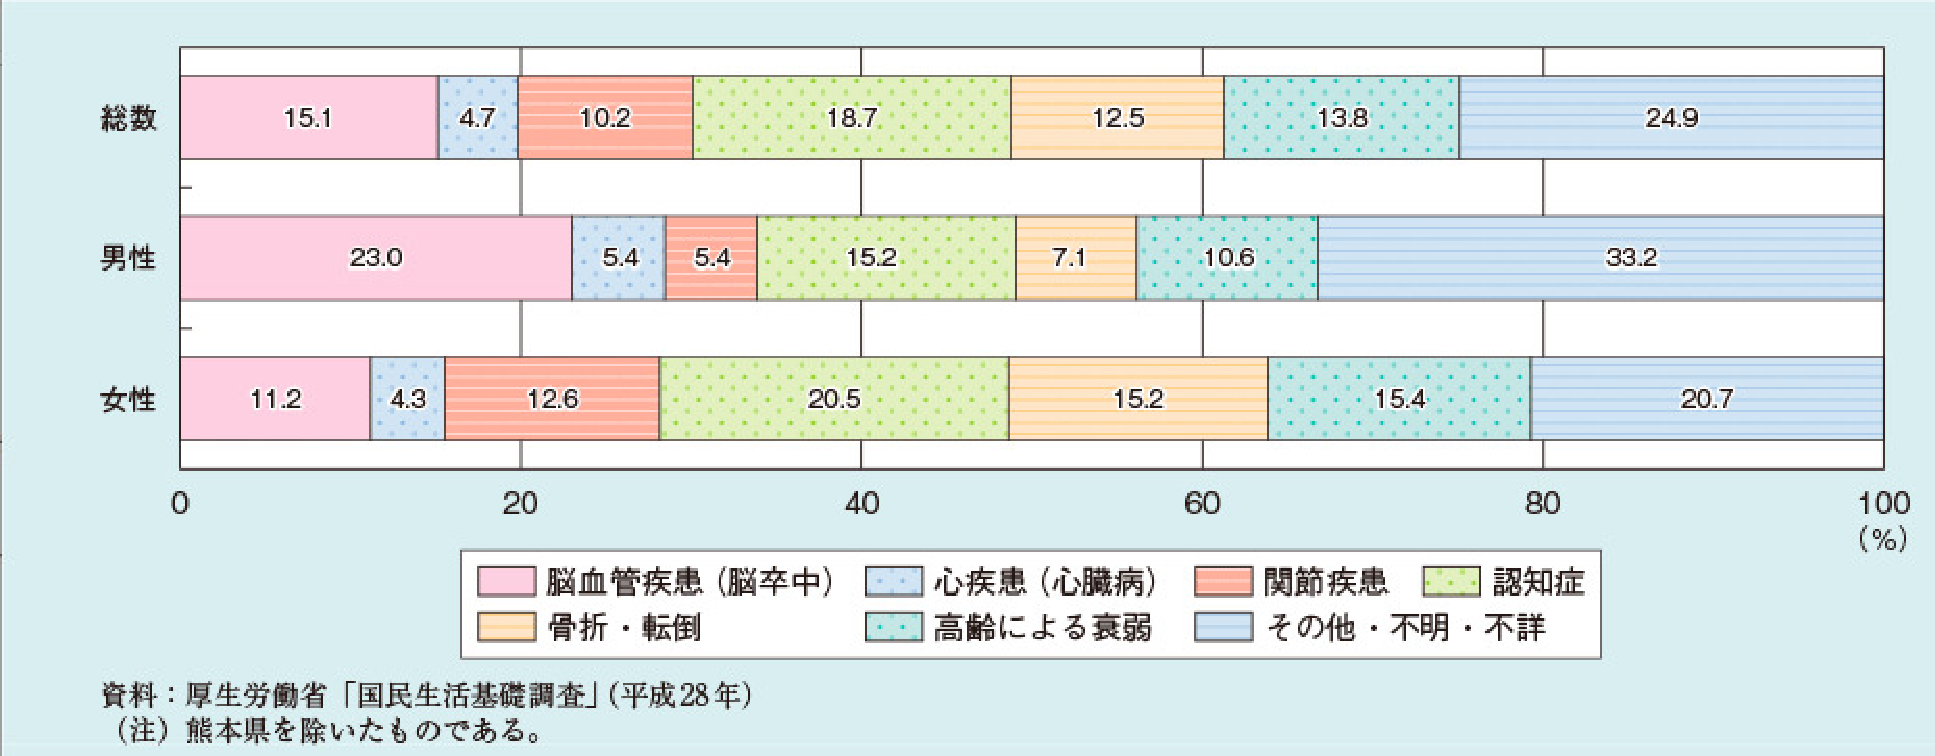
\includegraphics[width=140mm]{fig/kaigo.pdf}
  \end{center}
  \caption{65歳以上の要介護者などの性別にみた介護が必要となった主な原因\cite{kaigogenin}}
  \figlab{kaigo}
\end{figure}
\\\ \ Shear wave elastographyでは, 音響放射力によってせん断波を発生させる. 高フレームレート計測法, ドプラ法によって変位分布を, 粒子速度分布からせん断は速度の伝播を観察できる. 音響放射力が生体内で一様であるとした時に, 音響放射力により生じる生体組織の変位は$\mu$mオーダーであるため, ドプラ法によって加圧前後の超音波信号の位相差から変位を計測する[4]. 変位分布は得られるが, 前述した通り音響放射力が生体内で一様であるという仮定を除くと, 音響放射力の強弱によって生体組織の硬さは定性的な評価しかできない.
\\\ \ Transient elastographyでは, せん断波を加振によって発生させる. 一般的に, 超音波プローブから発せられる超音波ビームの軸方向を伝播するせん断波を計測する事は困難であるが, Transient elastographyではビーム軸方向のせん断波の計測が可能である. 超音波ビーム軸上の変位およびせん断波速度の分布の時間変化をドプラ法などにより計測し, 最小二乗法を用いる事でせん断波の伝播速度を取得できる. そのため, 比較的一様な組織であれば定量的な組織の硬さを評価することができる. 
\\\ \ Shear wave elastographyおよびTransient elastographyは生体組織の硬さを比較的定量的に計測できるが, 以下のような条件が必要である\cite{elastography}.
\begin{enumerate}
   \item 対象は無限に大きく, 小さな領域で一様である.
   \item 体積は変化しない. 
   \item 密度はどこでも同じ
   \item 振動の減衰が起こらない. 
\end{enumerate}
したがって下肢組織などのように骨があり, 振動の減衰が起こりやすく, 組織が均質とは見なせない組織では超音波エラストグラフィ使用は適していない. したがって, 上述したような4つの条件を満たさずとも組織の機械的特性を計測できる技術は, 生体組織の健康状態の理解に直結する. 以上に述べたことからも, 本研究の目標である定量的な下肢組織の健康状態の計測を可能にする超音波診断装置の開発には大きな意義があると考える. 次節にて超音波を用いた診断装置の技術について詳しく述べる. 
\begin{figure}[H]
  \begin{center}
    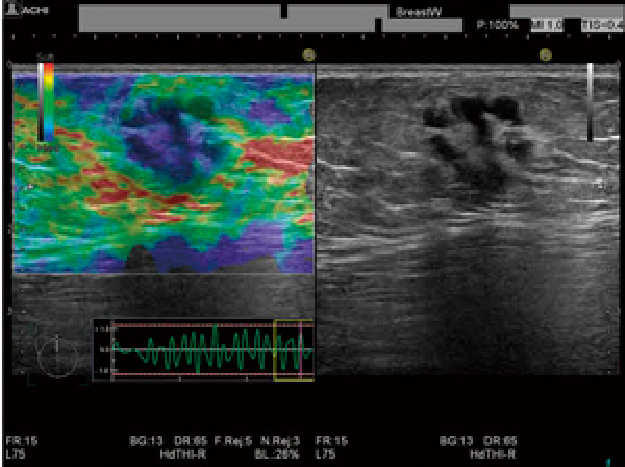
\includegraphics[width=75mm]{fig/elastography2.pdf}
  \end{center}
  \caption{エラストグラフィと断層画像}
  %http://www.innervision.co.jp/sp/feature/interview/201304
  \figlab{echo02}
\end{figure}

\section{超音波診断装置}
超音波を用いた生体の断層画像を取得する技術には, 超音波パルスエコーイメージングと超音波CTがある. 超音波を用いた医用画像は, ディジタル計算機の登場で飛躍的な進歩を遂げた, 問題点はまだ残されている. パルスエコーイメージングでは, 以下のような欠点がある. 
\begin{enumerate}
   \item 超音波は骨の透過性が低いため, 骨のある複雑な組織では正確な診断ができない.
   \item 超音波エコーではプローブを用いるため, 術者の技能によって取得画像の質が左右されてしまう.
\end{enumerate}
パルスエコーイメージングは, 超音波の反射を利用した技術であるが, 超音波CTは反射波だけでなく透過波も利用できる. 1976年, Greenleafらは透過波を用いて乳棒細胞の音速と減衰率を数値化し, 乳房の音響特性を測定した\cite{onkyou}. これにより. 音速を減衰率の関数としてプロットすることで良性腫瘍と悪性腫瘍を識別できることが示された.
\\\ \ 近年のコンピュータの発達により, 超音波CTは臨床応用が目指せるようになった. Duricらは\figref{hansha_0}に示すようなリング状の超音波の送受信素子が配置されたトランスデューサを上下に動かすことにより乳棒全体のデータ収集を行うCURE(Computed Ultrasound Risk Evaluation) と呼ばれる診断装置を開発し, 臨床試験を行なった\cite{cure1}, \cite{cure2}. リングアレイトランスデューサの直径は200mm, 素子数は256であり, 水槽内のレールに沿って上下動する. データ収集は5分程度で完了する上, 患者はベッドにうつ伏せに寝て乳棒を水槽内に挿入するだけでいいため非侵襲性である. パルスエコーイメージングとは異なり, 術者によって取得画像の差異が出ないという利点もある. \figref{hansha_1}にCUREによって得られた乳房の診断画像を示す.
\begin{figure}[h]
  \begin{center}
    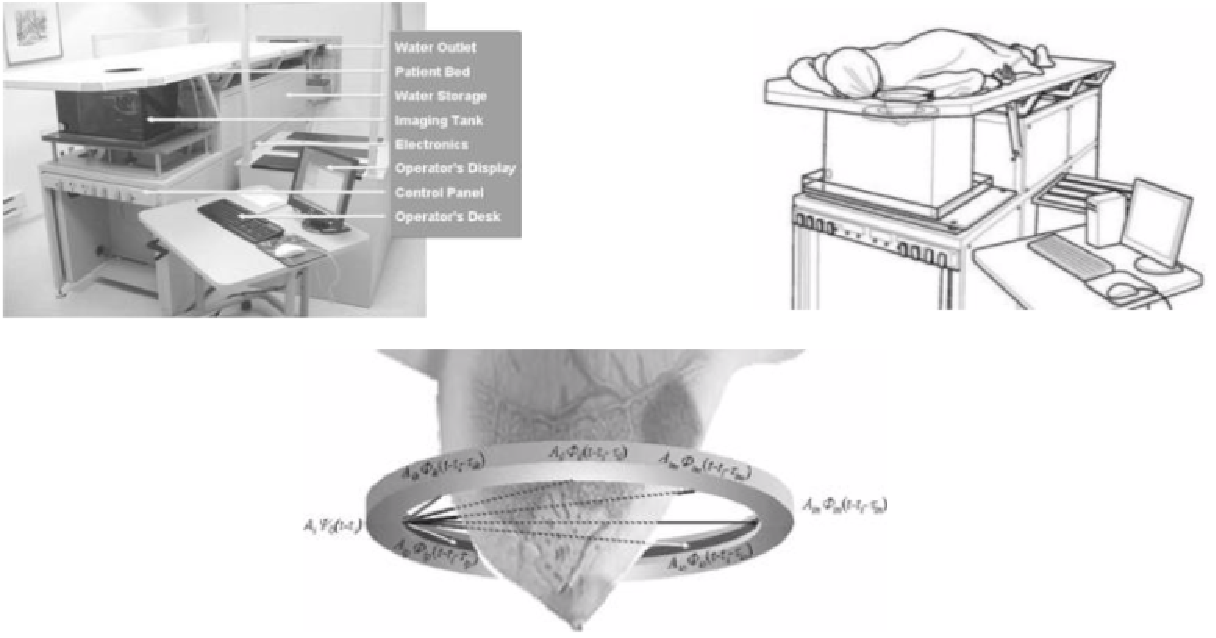
\includegraphics[width=110mm]{fig/curesystem.pdf}
  \end{center}
  \caption{CUREシステム}
  \figlab{hansha_0}
\end{figure}
\begin{figure}[h]
  \begin{center}
    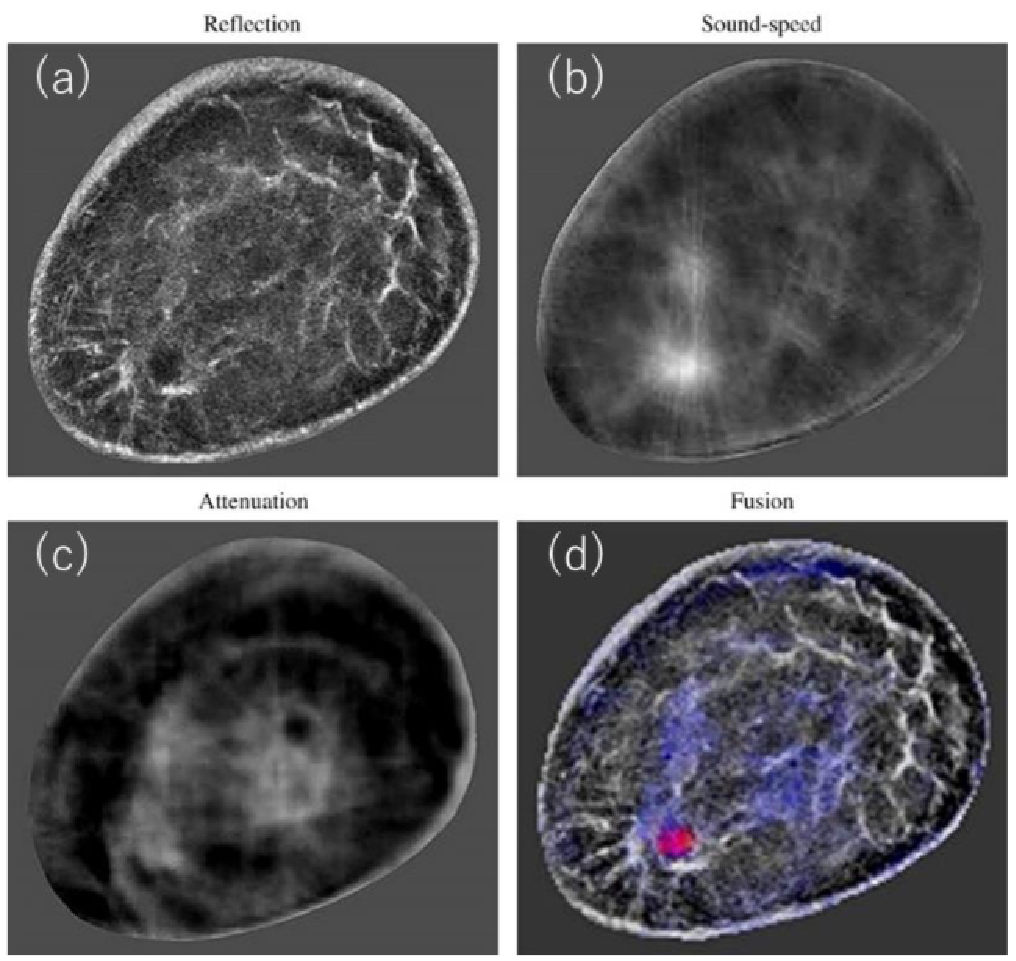
\includegraphics[width=75mm]{fig/curedansou.pdf}
  \end{center}
  \caption{CUREによって撮像された乳房の断層画像}
  \figlab{hansha_1}
\end{figure}
\section{リング型アレイトランスデューサ} 
 超音波CTを運用する上で必要なプロセッサは半導体技術の発展により高速度演算を可能にした. また超音波CTは安価で, MRIなどと比べて非侵襲的な診察が可能である.技術的進歩と需要が相まって, 超音波CTの機能を高めることの重要性は増している.  本研究では, リング型アレイトランスデューサ超音波CTを用いた下肢組織の定量的な診断装置の開発を目的としている(\figref{three}).以下でリング型アレイ超音波CTを用いた際の具体的な利点を3つあげる\cite{senpai}.
\begin{figure}[h]
  \begin{center}
    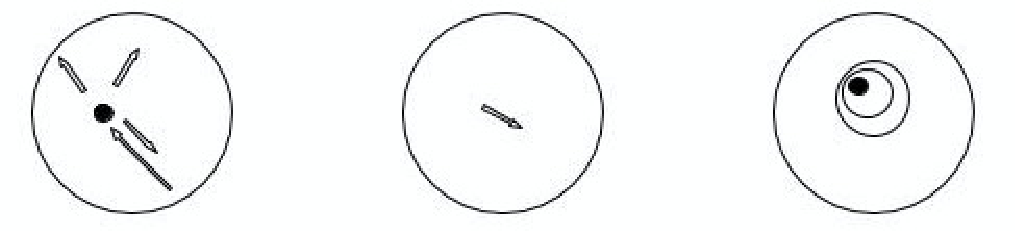
\includegraphics[width=120mm]{fig/three.pdf}
  \end{center}
  \caption{リング型アレイトランスデューサに期待される機能}
  \figlab{three}
\end{figure}
\begin{enumerate}
\item{\bf 透過, 反射, 減衰のトモグラフィ}
\\\ \ リングアレイを用いることにより, 反射波に加えて透過波を利用できる. しかし, 透過波については利用可能な臓器は限定される. また, 対象が骨や空気などの音響インピーダンスが大きな領域を含む場合は超音波はほとんど透過しないため, 透過波を用いることはできない. 
\item{\bf 任意方向のビーム伝播}
\\\ \ リング状に並んだ素子の内, 素子の選び方によって方向の異なる超音波ビームを形成することができる. これにより, 音響放射圧を多方向からかけることができ, 放射圧エラストグラフィにより組織の異方性を調べることができる. また, 血流ドップラー計測の多方向化など, 超音波による速度場計測が高度化する. 
\item{\bf 無限開口ビーム, 回折角=0}
\\\ \ 図 1. に示すのは, リング型振動子と球面型振動子からそれぞれパルス超音波が送波される際の超音波ビームである. 球面型振動子では焦点が広がっているのに対して, リング型振動子では完全に1点に収束している. このことから, リングアレイは理想的な点広がり関数を持ち, 任意形状の治療ビームの形成や, 従来型の診断プローブを用いた画像に見られたスペックルの存在しない診断画像が期待される. 
\end{enumerate} 
以上のように, リング型アレイ超音波CTには機能的には大きな利点があげられる.  計測対象である生体組織に骨があるということを考慮した上でさらなるリング型アレイ超音波CTの改善を目指す. 

\section{研究目的}
本研究の目的はリング型アレイトランスデューサ超音波CTを用いて下肢組織の健康状態を生体組織上を伝播するせん断波観察することで定量的に評価する診断装置の開発である. 前述のような診断装置の開発を実現するために, 以下の2つの課題に取り組む. 
\begin{enumerate}
   \item 下肢組織の断層画像の画像再構成の改善
   \item 下肢組織を加振した際の腱や筋肉を伝播するせん断波の計測方法の提案
\end{enumerate}
具体的には, 以下のようなシミュレーションおよび, 実験を行う.
\begin{enumerate}
   \item 下肢組織の断層画像の画像再構成をシミュレーションと実験のデータを比較.
   \item せん断波の伝播に伴い生じる, ひずみの伝播をトラッキングする手法を検討
\end{enumerate}
1. については, 下肢組織の形状を模したモデルを2つ作成し, それぞれについてリング型アレイ超音波CTでシミュレーションする. その際に得られた断層画像から生体組織の機械的特性, 考察しシミュレーション結果の画像処理の改善に取り組む. 2. については, まずは弦などをファントムとして加振した際のせん断波の伝播の様子をリアルタイムで超音波エコーによって観測し, 最終的にリング型アレイ超音波CTで伝播の様子を観測するが, リング型アレイ超音波CTはリアルタイムでの撮像ができないため, 得られた断層画像から対象物をトラッキングする手法を提案する. 

\section{本論文の構成}
 第1章では, 本研究の目的となる社会的, 技術的な背景および, 超音波CTを研究手法として用いることの有用性, リング型アレイトランスデューサの可能性について述べた.
\\\ \ 第2章では, 本研究において必要となる超音波やエラストグラフィなどに関する基本原理について述べる.
\\\ \ 第3章では, 先行研究を
\\\ \ 第4章では, リング型アレイトランスデューサを想定したk-waveによるシミュレーションの画像再構成手法に関する検討について述べる.
\\\ \ 第5章では, 本研究で試作したせん断波発生装置と, せん断波を発生させた時のファントムの挙動およびエコーデータから画像再構成された画像についての考察を述べる.






